\chapter{Introduction}
\label{Introduction}

%I first want to introduce the idea quickly, similar to an abstract. How online sports betting is a big growth industry, how esports are developing big time, how popular it is for people to bet on these esports matches. Then I want to specify how the algorithms used by sports betting companies are clouded in mystery - it's quite difficult to predict the outcome of sports events, and this is no different with esports. Statistical techniques are required, and the large amount of data genered natively by digital 'sports' make it a natural contender for analysis using machine learning techniques.
%
%• Start with a striking statistic or fact to grab attention about the growth of online sports betting and the popularity of esports. Highlight the mystery and complexity behind the algorithms used by betting companies.

\section{Background and context}

The rapid technological development of the 21st century has ushered in a digital transformation of most industries \cite{wef-tech}. The sports betting industry is no different. Placing a bet on the outcome of a sports match is now only a few quick taps away, as droves of online sports betting companies compete to take your wager. Electronic banking facilitates near instantaneous deposits and withdrawals between the user and the bookmaker, and the slew of odds and other betting options are generated 24/7 by computers running statistical models and complex algorithms. All of these advancements have made betting quicker, easier, and more accessible to an ever-expanding market of bettors \cite{structuresportsbetting}.

In a similar vein, the viability of \textit{electronic sports} relies on the uninterrupted functioning of an ensemble of technologies: complex computer hardware and peripherals providing the physical interfaces for the gameplay, the games themselves being the top layer of a highly-advanced software stack, and the high-speed, low-latency networking infrastructure that connects each player to one another in a virtual arena \cite{proesports-book}. With the sudden rise in popularity of this new form of competition, bookmakers have been quick to capitalise on a new market and offer betting opportunities for the outcomes of esports matches \cite{sizesportsbetting}.
 

\subsection{Online sports betting}
\label{background-bet}

Sports betting is a form of gambling whereby the bettor places a monetary wager on the outcome of one or more sporting events \cite{sportsbettingworld}. If the outcome(s) materialise, the bet is won and the bettor receives the value of their wager multiplied by the odds offered by the bookmaker. The odds for a given event are calculated by odds compilers, who analyse historical data and employ statistical techniques to accurately predict the probabilities of different outcomes \cite{oddscompiler}. The mathematical reciprocal of these probabilities determines the odds. To increase their profitability, bookmakers then decrease the odds slightly for either outcome. This difference between the compiled and offered odds is known as the bookmaker's margin \cite{margin}.

It is not known precisely when the practice of sports betting began, however sources claim that the Greeks would bet on the Ancient Olympic Games. The practice later appeared in Rome, where chariot racing and gladiator battles became the subject of the bets \cite{historybetting}. Betting on horse races was a popular activity in the United Kingdom by the early 18th century, and soon spread throughout the developed world \cite{historybetting-lamb}. By 1890, the United States boasted over 300 legal horse racing tracks, with horse race betting becoming a favourable pastime of the upper class. In the US, the industry was heavily regulated, and outright banned in 1910 \cite{historybetting-gray-1}. Regulations evolved over time, and the first government-sanctioned, brick-and-mortar sportsbook opened in Las Vegas in 1949. These businesses were known as 'Turf Clubs', and accepted bets on a number of professional sports, including the National Football League (NFL), National Hockey League (NHL), Major League Baseball (MLB), and National Basketball Association (NBA) \cite{historybetting-gray-2}.

The era of online sports betting began in 1996, when an Austrian-based sports book used the internet to legally connect sports bettors and bookmakers. On January 17th, 1996, the first online wager was made when Jukka Honkavaara bet \$50 on a football match: the first online sportsbook, Intertops (now known as Everygame), offered 1.04 odds for Tottenham Hotspurs to beat Hereford United. Though Honkavaara's winnings only amounted to a modest \$2, this event was nevertheless significant, as it marked the birth of the online sports betting industry \cite{historyonlinegambling}. 

Although regulations have hampered the industry in the US significantly, by 2023 the global market value of sports betting has grown significantly to 243 billion US dollars \cite{structuresportsbetting}. It currently accounts for over 40\% of global gambling revenue around the world - more than casinos, lotteries, and other forms of gambling \cite{sizesportsbetting}. Much of this growth can be attributed to the digitisation of the industry, which has led to increased access to and availability of betting opportunities. In 2018, the federal ban on sports betting in the US was lifted, and today it has been legalized in most states \cite{legalbettingtracker}. Furthermore, the industry is expected to grow significantly in Asia and Africa as laws surrounding sports betting become more relaxed and access to the online betting platforms improves \cite{structuresportsbetting}. The modern features and mechanics of the online betting industry will be further explored in the next chapter.

\subsection{Electronic sports}

The fastest-growing sports market, in terms of betting volume, are \textit{electronic sports}, also known as esports \cite{sizesportsbetting}. Esports are video games played in a competitive setting \cite{arcade}. The practice started in the 1970s and 80s on the floors of public arcades. The best players would rise to the top of persistent high-score leaderboards in their favourite titles like \textit{Space Invaders}, \textit{Pac-Man}, and \textit{Tetris} \cite{economicsjournalesports}. This type of competition was indirect, but by the 1990s, multi-player fighting games like \textit{Street Fighter} would see players pitted directly against each other. By then, the transition from arcades floors to home consoles and personal computers (PCs) was well under way, and the Local Area Network (LAN) party became the new battle arena. \textit{Doom} and \textit{Quake} marked the rise of first-person shooters (FPS) in this era. At the dawn of the 2000s, real-time strategy (RTS) games like \textit{StarCraft} and \textit{Warcraft} spawned the first professional leagues, legitimizing competitive gaming \cite{koreasports}.

High-speed internet became ubiquitous by the 2010s, and esports went mainstream. Multiplayer online battle arena (MOBA) games like \textit{League of Legends} and \textit{Dota 2} rose to prominence, and now boast tournaments with multi-million dollar prize pools. The largest esports prize pool to date was \textit{The International 2021} in Bucharest, Romania, with \$40 million US being awarded to the competitors \cite{growthofesports}. Although most are team games, some esports entail single players competing against one or more other players. In \textit{Fortnite}, only one player can emerge victorious in a 100-player 'battle royale', where the last surviving player wins. Kyle Giersdorf won at the Fortnite World Cup Finals 2019 at the age of 16, winning \$3 million US in the process. 

Today there are a substantial variety of game genres that are played professionally across the globe. Viewership figures for the major tournaments already rival traditional sports, and esports continue to grow and evolve without showing any signs of slowing down \cite{growthofesports}\cite{proesports-book}.  Esports revenues are expected to reach \$1.8 billion US in 2025, with a Compound Annual Growth Rate (CAGR) of 13.4\% between 2020 and 2025 \cite{growthofesports}. 

With a new form of competition, came a new form of gambling: esports betting. The industry initially developed in regulatory grey areas, such as the infamous CSGOLounge.com \cite{hardenstein2017skins}, which accepted wagers of hitherto unregulated virtual currencies and items, such as "skins" - tradable, in-game cosmetic items \cite{esportsgambling}. Skins and other virtual items have many of the same properties as non-fungible tokens (NFTs), often having unique identifiers, rarities, or characteristics which make them desirable in addition to their in-game utility. A significant market exists for these virtual items, with extremely rare skins being sold for thousands of dollars \cite{hardenstein2017skins}. 

The industry has been formalized over time, and it is now common to see esports alongside traditional sports on legal betting sites. Controversies still remain, however, as bookmakers frequently sponsor teams and tournaments, promoting online betting to a growing, and often young, population of spectators \cite{bettingsponsors}. Furthermore, the prevalence of sports betting can undermine the integrity of competition. A hallmark case of match-fixing occurred in 2015 \cite{matchfixing}, where a top American team, iBUYPOWER, purposefully lost a match they were heavily favoured to win. A number of players were later found to have received kickbacks in the form of valuable skins. This prompted Valve, the game developers, to take action to preserve the integrity of the game. All the players that were accused of "throwing" the match were banned from competing in Valve-sanctioned tournaments, effectively ending their careers as professional Counter-Strike players \cite{ibuypower}.

Counter-Strike (CS) currently dominates the esport betting market, with 56\% of all wagers in this segment being placed on CS matches \cite{abios_report}. There are also a number of online sites which track and collect data relating to these matches, such as HTLV \cite{hltv-about} and Liquipedia \cite{liquipedia-prizepool}. It is therefore an attractive esport to consider for this research.

\subsection{Overview of Counter-Strike}

The first version of Counter-Strike emerged in 1999 as a community-developed 'mod' (modification) for \textit{Half-Life}, the hit FPS developed by Valve Corporation. With its unique emphasis on team-work and co-ordination, CS quickly garnered attention from players. The following year, Valve hired the developers of the mod, acquired the intellectual property (IP), and subsequently launched CS as a stand-alone title \cite{retromag}. It did not take long for a competitive scene to emerge. The first tournaments were organized in Europe in 2001 by the Cyberathlete Professional League (CPL), with prize pools of ten to twenty thousand euros \cite{csmajors}. Since then, the game has soared in popularity over a number of iterations, and the quality and scale of competition has grown along with it. \textit{Counter-Strike 2} was released on the 27th September 2023 and played by over 30 million players in the first month \cite{cs2playercount}.

Over the last decade, CS has cemented itself as one of the major esports in the world. There are several competitive tournaments hosted by organizations like the Electronic Sports League (ESL), DreamHack, and Intel Extreme Masters (IEM). Leagues typically culminate in major in-person LAN events  where the best teams compete for their share of prize pools which regularly exceed a million dollars. Valve-sponsored Major tournaments are the pinnacle of the CS calendar and attract millions of concurrent viewers on streaming platforms in addition to a packed stadium of fans. The PGL Major event, pictured below, had a prize pool of \$2 million US and reached a peak viewership of 2.7 million spectators across multiple online platforms. \cite{pglliquipedia}\cite{pglarticle}. At present, the sum total of all CS tournament prize pools to date is over \$187 million US \cite{liquipedia-prizepool}.

\begin{figure}[h]
	\centering
	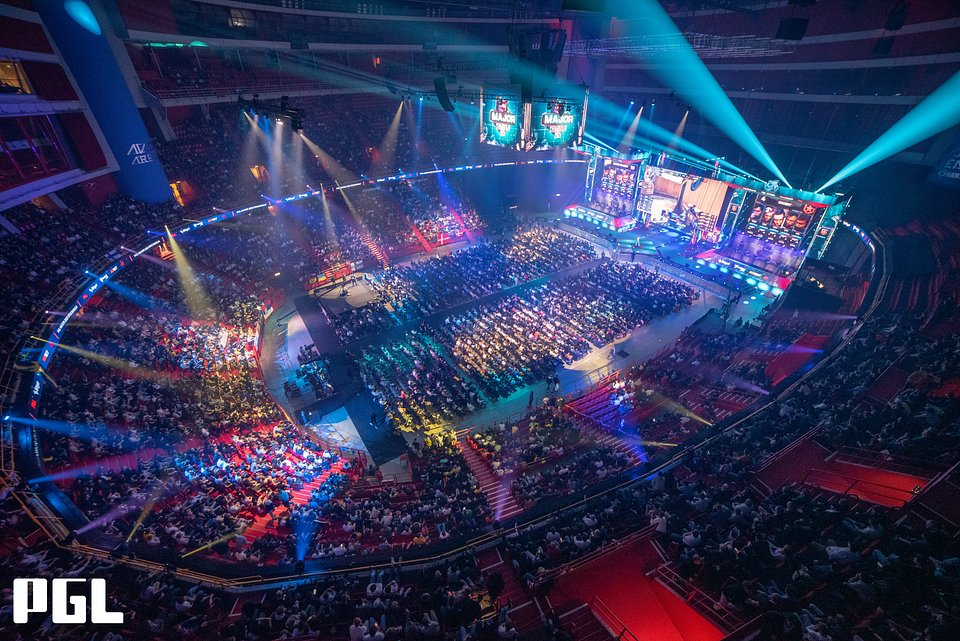
\includegraphics[width=\textwidth]{Figures/major.jpg}
	\caption{The 2021 PGL Major took place in the Avicii Arena in Stockholm, Sweden \cite{pglarticle}}
	\label{fig:major}
\end{figure}

\subsubsection{Gameplay fundamentals}

Counter-Strike is a PC video game played using the mouse, keyboard, and headset. Players assume the role of a soldier in a virtual 3D environment, which can run, walk, and jump by pressing keys on the keyboard. The mouse is typically used for two purposes: to control the direction and movement of the in-game field-of-vision, and for shooting, where cross-hairs at the centre of the player's screen act as the focal point for aiming. For effective communication, players co-ordinate their actions with their team-mates primarily through a headset with a built-in microphone. 

Although a number of versions have been released since its inception, the core game mode played in Counter-Strike, known as \textit{defusal}, has remained relatively unchanged. Two teams of five players each start each round on opposite ends of a virtual arena called a \textit{map}. One team plays the role of the Counter-Terrorists (CT), whose objective is to defend two bomb sites, A and B, from the opposing team, the Terrorists (T). The layout for the popular Counter-Strike map, Mirage, is shown in Figure \ref{fig:mirage}; the red zones highlight the bomb sites and the green zones are the spawn areas for either team. There are seven official maps played in competitive Counter-Strike.

\begin{figure}[h]
	\centering
	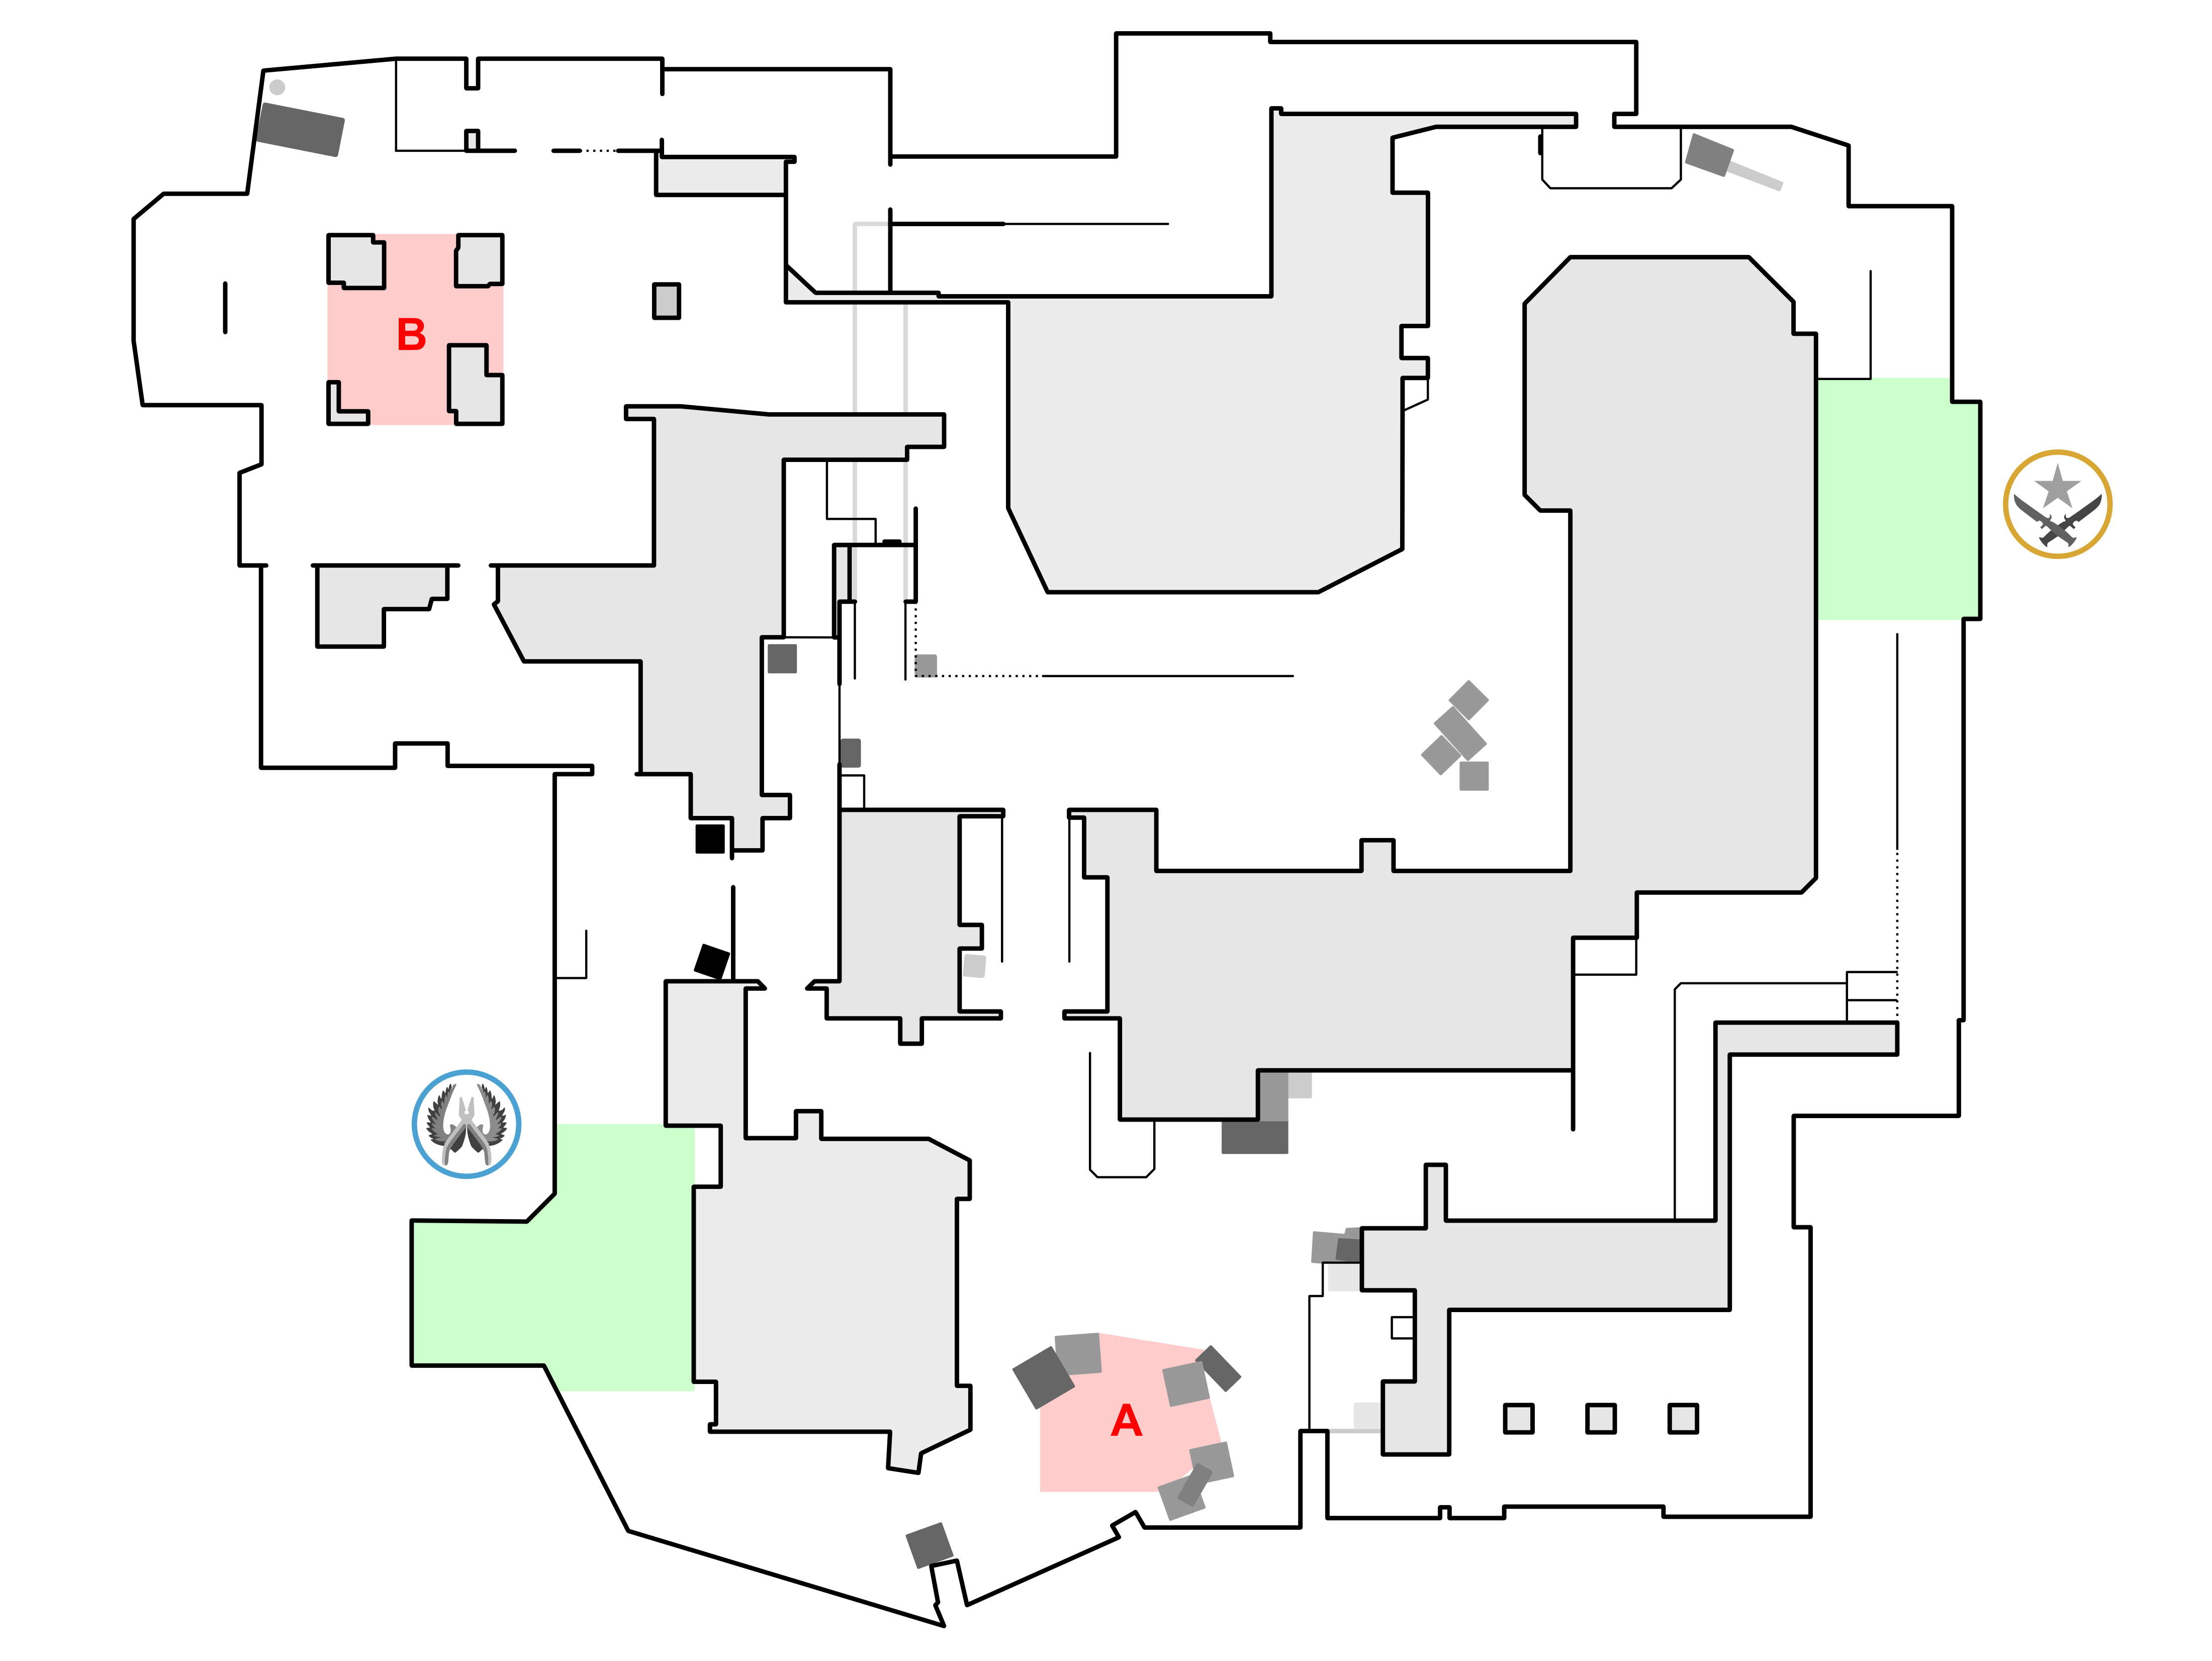
\includegraphics[width=0.9\textwidth]{Figures/mirage.png}
	\caption{Map layout for 'Mirage', showing spawn areas in green and bomb sites in red \cite{mapdiagram}}
	\label{fig:mirage}
\end{figure}

A map is played for best-of-24 rounds, with teams swapping sides after 12 rounds. This means that in order to win, a team must demonstrate superiority over their opponents in both attacking (as Ts) and defending (as CTs). The first team to win 13 round wins the map. In the event of a tie (12-12), the map continues in best-of-6 round \textit{overtime} phases, with sides swapping every 3 rounds, until a winner is decided.

Each round, spanning 1 minute and 55 seconds, is a high-stakes scenario as each player has only one life. Eliminated players have to spectate their living team-mates until the next round. Rounds can be won in four ways: by (1) eliminating the entire enemy team, or, if playing as Terrorists, by (2) detonating a bomb on one of the bomb sites. Once a bomb is planted, the round timer changes to a 40 second countdown until detonation. The Counter-Terrorists can win rounds either by (3) successfully defending both sites for the duration of the round, or by (4) retaking the bomb site and defusing the bomb after it has been planted. Players begin each round with 100 health points (HP). Damage is measured in HP and can be inflicted using a variety of weapons and grenades. There is no way to replenish HP during a round.

\subsubsection{Strategy and team economy in Counter-Strike}

Different strategies (\textit{meta}'s) evolve for attacking and defending the various points on each map, with players learning which positions are optimal to hold with different weapons, how, when, and where to throw their \textit{utility} (smoke, flash-bang, high-explosive, and incendiary grenades), and how to move around the map as the round unfolds. All positions on a given map are named such that players can immediately communicate critical gameplay information to their teammates over the course of a round. Success in Counter-Strike relies on efficient team-work as much as mechanical skill, as player actions need to be co-ordinated in order to optimally assist one's teammates. This can be in terms of positioning (e.g. setting up a cross-fire at a choke point\footnote{A choke point is a small part of the map near each bomb site which, if controlled, gives either team a tactical advantage.}, or moving to help bolster the defence at a bomb site which is being attacked) or in terms of utility usage (e.g. throwing an incendiary grenade at a choke point in order to slow down an attack, or throwing a flash bang to allow a teammate to take control of a position). 

Players are rewarded with in-game money for getting a kill, planting or defusing the bomb, and winning or losing a round. Winning a round is rewarded with far more money than losing a round, however this amount (the \textit{loss bonus}) grows with each consecutive round loss. Money is spent to purchase weapons and equipment at the start of each round. If a player survives the round, they retain whatever equipment they had into the following round. Each team therefore has a monetary balance, known as the team economy, which fluctuates throughout the duration of a map. A stronger economy means you can purchase stronger weapons and more equipment. A weaker economy might relegate your team to just buying a few pistols and practically forfeiting a round in order to save funds for the following round. Sound economic strategy is thus critical to success in Counter-Strike.

At the start of a half, both sides have almost no money and so duel with only pistols. The \textit{pistol round} is quite crucial, as it initiates economic momentum for whichever team wins it. In some exciting cases, teams will defy odds and trade the initial rounds back-and-forth, leaving the economic balance undecided. A game can become extremely tense if both teams have precarious economies near the end, as the outcome is undecided and the stakes get progressively higher. 

The state of each team's economy is a good predictor of their ability to win a given round. This is the total team balance as well as their current loss bonus; teams earn progressively more money with consecutive round losses up to a cap of \$3400 after 5 losses in a row - matching the round-win bonus. A team with the funds to 'full-buy' will almost always win a round against a team that is saving their money in an \textit{eco} round where  they don't purchase anything other than pistols. A \textit{semi-buy} is a middle-ground, used to save enough funds to ensure a \textit{full-buy} the following round, but still giving the team a fighting chance. These distinctions therefore refer to the strength of the weapons and amount of utility grenades that can be purchased in each round.

An example of the economy for two teams over the course of a map is shown in Figure \ref{fig:economy}. The lines corresponds to either team's balance, and a coloured icon represents a round won by the CTs (blue) or the Ts (orange) respectively. The horizontal lines are thresholds that indicate the health of the economy, indicated as eco, semi-buy, and full-buy. Note that the pistol rounds take place in rounds 1 and 13, and teams switch sides in round 13 which results in the round-win icon colour switching.

\begin{figure}[h]
	\centering
	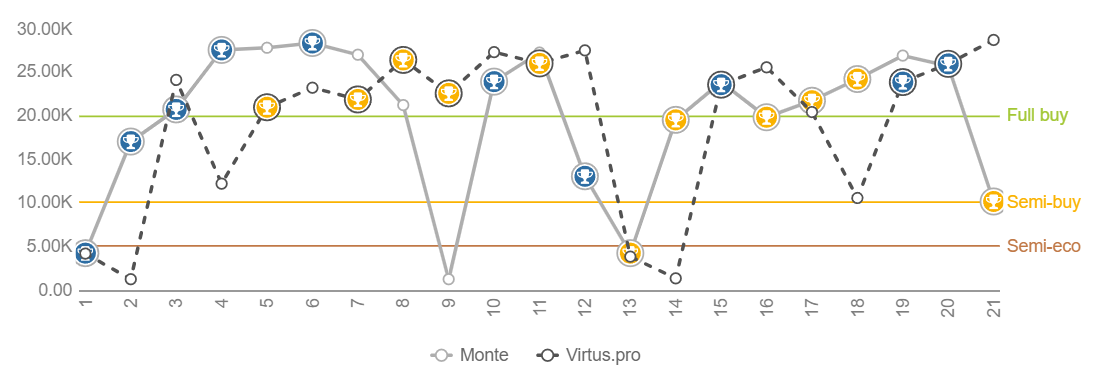
\includegraphics[width=\textwidth]{Figures/economy.png}
	\caption{A graph showing the economies of two teams over the course of a map \cite{vpmatch}}
	\label{fig:economy}
\end{figure}


\subsubsection{Professional Counter-Strike}

The local area network (LAN) is the most competitive environment possible, as all players have the same, virtually instant network latency and there is no possibility for gameplay 'lag'. They play under the same conditions and use identical computer hardware (except for their keyboards and mice). Tournaments played "on LAN" represent the pinnacle of competitive Counter-Strike, with teams flying all over the world to attend these events. Teams qualify for LAN events either through invitation (due to their position in the world ranking), or by placing sufficiently high enough in qualification rounds that are normally played online.

Professional CS matches are played in a best-of-1 (BO1) or best-of-3 (BO3) maps format. The grand final for bigger tournaments are occasionally contested in a best-of-5 (BO5) map series. Match lengths can vary greatly depending on the format and skill-disparity between competitors. A BO1 can be concluded in 20 minutes if one team dominates the other. In extreme cases, a BO5 grand final between two evenly matched giants can become a five-hour affair as tightly-contested maps get traded back-and-forth. The most common format is the BO3, where the match winner is determined over 2 or 3 maps which last roughly 40 minutes each.

Although CS is a methodical and tactical team-based shooter, it is highly dynamic in the short, medium, and long term. During individual rounds, players must make split-second decisions to react to events as they unfold. Over the course of a map of 24 rounds, teams need to learn and adapt to their opponent's habits in order to exploit their weaknesses. Between matches, teams will often adopt and improve strategies from other teams by reviewing their gameplay recordings, or come up with entirely new approaches to counter a certain prevailing strategy.

Teams have coaches whose role is to identify these trends mid-match and suggest appropriate countermeasures. The better-resourced teams employ analysts who review their opponent's games and develop strategies in advance. Competitive CS is mentally demanding, so teams often have sports psychologists to keep the players operating at peak performance \cite{sportspsych}. Throughout the match, coaches must ensure their players maintain composure. As discussed earlier, the longer format matches can become a battle of mental endurance. This has led to some controversy surrounding esports players and the use of stimulants like Adderall \cite{adderall}.

\subsubsection{Data in Counter-Strike}

Every second of CS game generates a wealth of data; in previous versions of the game, the 'tick rate' is the frequency at which each player's game client is synchronized with the server. Professional matches were played exclusively on '128-tick', which means there were 128 snapshots of the game being generated each second, containing every minute detail of the game: each player's precise location on the map, the direction at which they are aiming, and the state they are currently in - moving, jumping, shooting, throwing a grenade, reloading, switching weapons, planting or defusing a bomb, shooting or being shot at. At any given point there can be a number of smoke grenades deployed on a map, a high-explosive grenade being lobbed towards an enemy position, or an incendiary grenade temporarily blocking a choke point. 

With the introduction of CS2's sub-tick system, the granularity of data has been further enhanced, as player movements and interactions can now be recorded in-between ticks using an interpolation system. It should be evident that there is a tremendous amount of data generated in each map played. This gameplay data is stored in a \textit{demo file}, which can be replayed at a later stage or processed for data analysis.

A number of statistics can be generated by processing these demo files. For example, player performance can be measured by the number of kills, deaths, assists, average damage per round (ADR), and weapon accuracy. Free online tools like Leetify rate all players from the data in their match demo-files. They report statistics such as \textit{cross-hair placement precision}, which refers to the degree deviation of the cross-hairs from an enemy who comes into view, \textit{time-to-damage}, which is the number of milliseconds between seeing an enemy and inflicting damage, and \textit{headshot accuracy}, which is the proportion of kills attained by lethal headshots. \textit{Clutch} statistics refer to the percentage of rounds won where a player is last alive on his team versus 1, 2, 3, 4, or 5 opponents. All of these data points help to paint a descriptive picture of a player's contribution to their team's success or defeat. That said, some roles, such as \textit{support} or \textit{in-game leader} (IGL) help their team in ways that are harder to quantify.

Team performance is usually measured by their win-rates on the various maps. Teams have preferred maps, and most also have \textit{perma-bans} which they never play. In a BO3 series, teams will decide which of the 7 maps to play through a veto process; this always follows a ban-ban-pick-pick-ban-ban-decider sequence. There are therefore trends in which maps a team will play and will avoid. A map-veto which favours one team in an otherwise equal match-up can therefore make for a favourable bet. \label{vetoprocess}

All these statistics are prominent features of a professional broadcast; for example, commentators will refer to the weapon accuracies when contrasting the snipers of opposing teams. Dominant teams can go on significant match or map-win streaks, which adds further tension to tight matches. On certain broadcasts, there is a round-win prediction percentage which sways depending on the round economy and number and health of players alive on each side.


\subsection{Machine learning}

\textit{Machine learning} (ML) is an interdisciplinary field, spanning computer science, statistics, and data science. It refers to the development and study of statistical algorithms that can learn from data and generalize to unseen data \cite{mlbook}. It is fitting that the term was coined in 1959 by Arthur Samuel, who, while working at IBM, invented a program to calculate the chances of either side winning in the game of checkers \cite{mlcheckers}. In the last two decades, improvements in computational power has allowed the field to develop from a theoretical concept into a practical technology with widespread commercial use. Today, machine learning methods are employed across a plethora of industries, including health care, manufacturing, education, financial modelling, and more \cite{mltrends}.

ML is considered a subset of artificial intelligence (AI), as many of the algorithms imitate the way that humans learn \cite{mlibmdef}. ML techniques are used for the development of software that perform computer vision, speech recognition, natural language processing, and much more. It is normally far easier to train a system using large amounts of data than it is to explicitly program it to anticipate a desired response for all possible sets of inputs. This makes ML an effective tool for many "big data" applications \cite{mltrends}.

There are three broad categories of machine learning paradigms, which differ primarily on the nature of the feedback available to the learning system. These are (1) supervised learning, (2) unsupervised learning, and (3) reinforcement learning. In \textit{supervised learning}, the system learns from data with known outputs. In other words, the goal is to learn how to map a series of inputs to a series of outputs. It is commonly found in applications like image recognition. In \textit{unsupervised learning}, there are no known output labels and the goal is to learn hidden patterns or structures in the data. An example of this is customer segmentation in marketing. Finally, in \textit{reinforcement learning}, an agent tries to achieve a goal in a dynamic environment known as the problem space. As it navigates the problem space, it is rewarded for good responses and punished for bad ones. The system attempts to optimize the proportion of good responses. This ML paradigm applies to areas such as robotics and game playing.

For this research, the objective is to predict the probability of either team winning given a large dataset of information about two teams. The problem can be expressed as predicting whether Team A will beat Team B, with a binary answer of no, they lose (0), or yes, they win (1). Given that the input data is derived from a large dataset of match records with known outcomes, supervised learning techniques are pertinent. In the subsequent chapter algorithms which have shown promise in sports analytics will be explored.

\section{Research problem}

The techniques used by bookmakers to compile betting odds are not well-represented in the literature. Furthermore, esports betting is a high-growth segment of the market, and professional Counter-Strike matches drive a significant amount of online betting activity. Counter-Strike is a complex esport, with several factors making it difficult to predict. While existing literature has explored machine learning in traditional sports, its application in esports, particularly in Counter-Strike match prediction, remains underexplored. Fortunately, an abundance of data is generated during these matches by virtue of their digital nature, making them an ideal subject for investigation. This study aims to explore whether machine learning techniques can be used to make accurate predictions, and by extension, betting odds estimations, for professional Counter-Strike matches. 

\section{Research objective}

The primary objective of this study is to develop a model that can estimate the odds of either team winning for any given match of professional Counter-Strike. This objective can be broken down into a number of smaller objectives:

\begin{enumerate}
	\item Review the literature on the technology used in the sports betting industry, and on the application of machine learning techniques for sports prediction
	\item Gather a significant dataset of historical data for professional Counter-Strike matches
	\item Identify and generate relevant features from the historical match data
	\item Train a selection of supervised learning models to generate probability estimates and betting odds for either team winning
	\item Measure and compare the performance of each model using classification accuracy and F1-score, and identify the most relevant features for match prediction
	\item Compare the betting odds generated by the models to actual historic betting odds
\end{enumerate}

\section{Scope and limitations}

Although this minor dissertation is concerned with the esports betting industry, it is not feasible to create a model that can predict the outcome for every esport. This is because there are a large variety of esports with different competition rules, gameplay factors, and players. It was therefore decided to focus on one specific esport: Counter-Strike.

In Counter-Strike, there are many betting opportunities beyond just the match winner. As discussed earlier, matches are played in different formats consisting of one or more maps of gameplay. Bettors are often given the opportunity to place bets on which team will win the current map, which team will win the pistol round for a given map, or which team will simply get the first kill of a map. Although map-specific data is used for feature selection, the objective of this research is to quantify probabilities for winning the entire match. The most common match format is Best-of-3 maps, which will be considered the default for this project.

Furthermore, in recent years, live or in-play sports betting has become popular; bettors can make bets while a match is being played, and often cash-out their existing bets for some discounted return. Bookmakers offer dynamic odds which rely on live match analysis. While some research has been done in the field of real-time match prediction, this project will focus purely on predicting the overall match outcome using only historical information, i.e. before the match has begun.

Finally, bookmakers can to some extent monitor market dynamics as they know which bets are being made. They can therefore factor in the market expectations by adjusting the odds offered on different outcomes using the betting information available to them. This data is privy to the bookmakers and will thus not be included in the modelling process.

\section{Ethics approval}

This project was approved by the Commerce Research Ethics Committee with code COM/00541/2023. The approval letter has been included in Appendix \ref{dix:ethics}.

\section{Structure}

This dissertation is comprised of five chapters. The introduction covers the background knowledge relevant to the topic, defines the research problem, and establishes the objectives. Thereafter,  existing research on the esports betting industry and data-driven match prediction is covered in the literature review. 

The third chapter precisely describes the methodology employed to achieve the research objects: how the data is collected, stored, processed, analysed, and used to generate the features. The models selected and the techniques used to train them are all described in this chapter. This chapter is concluded with a description of the script which takes a match input and generates the betting odds. 

The penultimate chapter is a discussion of the results obtained in the modelling process, and how well the objectives were met. Finally, a conclusion summarizes the key findings, limitations, and suggestions for areas of future research.